%
% Another appendix chapter
\chapter{Variable Height Inverted Pendulum Capture Regions}\label{chap:regions}
Using simple models for a walking humanoid robot, it has been a common approach to study point-foot placements where it is possible to come to a stop. Such a point-foot location is referred to as a \textit{capture point} in \cite{pratt2006capture}. In the case of the \ac{LIP} model, only one capture point exists: the \ac{CP}. If a torque controlled flywheel is added to this model, a control input is available and reaching a set of capture points will become possible. This set of capture points is referred to as a \textit{capture region}, also called a stability region in \cite{stephens2007humanoid}. A control input however can also become available without addition of a flywheel to the \ac{LIP}.


Taking away the height constraint of the \ac{LIP}, results in the \ac{VHIP}. Height variations can be used to control the capture region. Equation \ref{eq:dynamicscaronstyle}, written in \ac{2D}, reads as follows:
\begin{equation}
	\label{eq:vhip2d}
	\ddot{x}=\frac{g+\ddot{z}}{z}x.
\end{equation}	
In this chapter, capture regions are derived by adding constraints to the model above. Recovery is considered within the current step, which is equivalent to `0-step' capture in \cite{koolen2012capturability}. A capture point is denoted as a positive value, while the initial state of the above model is set to $x_0<0$, $z_0>0$, $\dot{x}_0>0$ and $\dot{z}_0=0$. So if $x_0$ is a capture point, this is denoted as $x_{cp}=-x_0$.



%Unilateral
\section{Unilateral Contact Constraint}
The assumption is made that the robot can only push on the ground with its legs. This introduces a constraint of contact unilaterality. The downward acceleration of the point-mass is constrained by gravity acceleration, and the constraint $\ddot{z} \geq -g$ is added to the \ac{VHIP} model of Equation \ref{eq:vhip2d}.

Neglecting forces, the velocity of the point-mass can be instantly changed by an impact of the \ac{VHIP}. Writing Equation \ref{eq:vhip2d} in terms of instant velocity changes gives:
\begin{equation}
	\label{eq:vhipi}
	\dxi=\frac{\dzi}{z}x,
\end{equation}	
where $\dxi$ and $\dzi$ are the horizontal and vertical velocity change, resulting from an impact by the \ac{VHIP}.

For the first bound on the unilateral contact constrained capture region, the closest possible capture point is explored. Using Equation \ref{eq:vhipi} and that $\dot{x}_0+\dxi=0$ for a capture point, there exists an infinite vertical impact that results in the capture point approaching zero:
\begin{equation}
	\lim_{\dzi \to \infty} \xcpunif = \frac{z_0}{\dzi}\dot{x}_0 = 0,
\end{equation}
where $\xcpunif$ is the first bound on the unilateral contact constrained capture region.

For the second bound of the region, the minimum possible vertical acceleration of  $\ddot{z} = -g$ is used. With this vertical acceleration, the dynamics of the point-mass depend on gravitational forces only: the point-mass follows a \textit{ballistic} trajectory. After this ballistic trajectory, the mass can be stopped by an impact of the \ac{VHIP} at $z=0$. The time after which the point-mass touches the ground is:
\begin{equation}\label{eq:tbal}
	t_{bal} = \sqrt{\frac{2z_0}{g}}.
\end{equation}
The horizontal location at this time is:
\begin{equation}
	x_{bal}= \dot{x}_0t_{bal}=\dot{x}_0\sqrt{\frac{2z_0}{g}},
	\label{eq:xbal}
\end{equation}
where $x_{bal}$ is the ballistic touchdown point. This point is the second bound on the unilateral contact constrained region. Also, this point has a special relationship with the \ac{CP}:
\begin{equation}
    \xcpunis = x_{bal}=\sqrt{2}\xcplip
\end{equation}

%This can also be reasoned from a virtual leg force perspective, as no horizontal energy is subtracted from the point-mass during its travel. Using this problem formulation and inserting a final velocity in the \ac{LIP} orbital energy Equation \eqref{eq:Elip} gives:
%\begin{equation}
%   x_{bal}^2 = \frac{z_0}{g}\big(\dot{x}_0^2 + \dot{x}_f^2\big), 
%\end{equation}
%where $\dot{x}_f$ is the final horizontal velocity of the \ac{CoM}. If a ballistic trajectory is considered, the horizontal velocity is not affected until touchdown, so $\dot{x}_0=\dot{x}_f$. The solution to $x_{bal}$ is equal to Equation \ref{eq:xbal}.

The capture region spanned between these two bounds reads as follows:
\begin{equation}
\xcpuni \in \Bigg(0, \dot{x}_0\sqrt{\frac{2z_0}{g}} \Bigg],
\label{eq:xcpuni}
\end{equation}
where $\xcpuni$ is a unilateral contact constrained capture position. In \figref{fig:cpbal} this region and the \ac{CP} are visualized. With gray plots, made with the method of \cite{koolen2016balance}, it can be observed how the trajectories can become very high, when approaching the left side of the bound.  

\begin{figure}
\centering
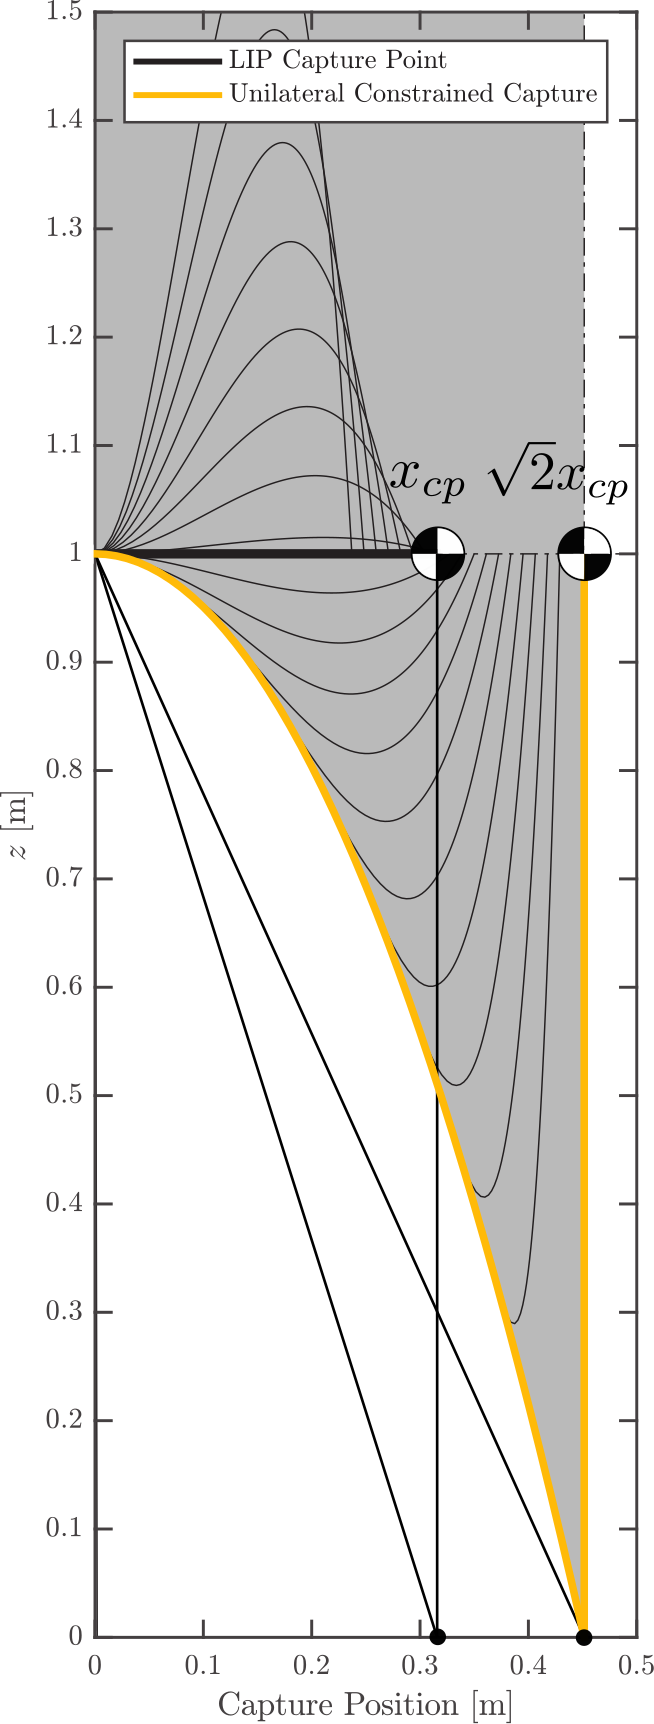
\includegraphics[width=3.0in]{STYLESTUFF/CPvsBalistic3.png}
\caption{Unilateral contact constrained capture region (gray area). The thin black lines visualize possible intermediate trajectories and are made with the method of \cite{koolen2016balance}.}
\label{fig:cpbal}
\end{figure}

%% Height Constrained
\section{Height Constraint}
To further constrain the \ac{VHIP} model, kinematic constraints are taken into account. Under the assumption that kinematic limits of the robotic system can be approximated with a minimum and maximum \ac{CoM} height, in this section a \textit{minimum} and \textit{maximum} height constraint are added to the unilateral contact constraint capture region of the previous section. The capture points that will be discussed are a combination of impacts, ballistic trajectories and \ac{LIP} capture trajectories, such that closed-form solutions become available. 

\subsection{Maximum Height}
With an initial vertical impact of the leg of such magnitude that the resulting apex of the point-mass does not violate the maximum height constraint, a capture position under a maximum height constraint can be derived. This capture point is computed using the vertical impact first, followed by a ballistic trajectory, after which the \ac{CP} at the maximum height is used.

To calculate the allowed size of the initial impact, the following equality of kinetic and potential energy is used:
\begin{align}
 	\frac{1}{2}m\dzi^2 &= mg\delta z_{max},\\
 	\dzi &= \sqrt{2g\delta z_{max}}, 
\end{align}
where $\delta z_{max}=\zmax-z_0$ is the height difference between the current and the maximum height. The initial horizontal velocity is influenced at the moment of the impact as follows:
\begin{equation}\label{eq:dotximpact}
	\dot{x}_{0,I} = \dot{x}_0-\frac{x_{cp,\zmax}}{z_0}\dzi,
\end{equation}
where $\dot{x}_{0,I}$ is the remaining horizontal velocity after impact and $x_{cp,\zmax}$ is the capture position following the maximum height constraint, to be determined. Note that at the moment when $z$ reaches $\zmax$ for the first time after the ballistic trajectory, $\dot{x}_{0,I}$ is unchanged as no virtual leg force is used. The duration of this ballistic trajectory is given by:
\begin{equation}
	t_{\dot{z}>0} =\frac{\dzi}{g},
\end{equation}
where $t_{\dot{z}>0}$ is the time that the height velocity is nonzero. The capture position under the maximum height constraint is calculated as follows:
\begin{align}
	x_{cp,\zmax}&=\bigg(t_{\dot{z}>0}+\sqrt{\frac{\zmax}{g}}\bigg)\dot{x}_{0,I},\\
			&=\bigg(\frac{\dzi}{g}+\sqrt{\frac{\zmax}{g}}\bigg)\bigg(\dot{x}_0-\frac{x_{cp,\zmax}}{z_0}\dzi\bigg).
\end{align}
Taking $x_{cp,\zmax}$ to the left-hand side leads to:
\begin{align}
	 \Bigg(1+\bigg(\frac{\dzi}{g}+\sqrt{\frac{\zmax}{g}}\bigg)\frac{\dzi}{z_0}\Bigg)x_{cp,\zmax}& =		\bigg(\frac{\dzi}{g}+\sqrt{\frac{\zmax}{g}}\bigg)\dot{x}_0,\\
	 x_{cp,\zmax} & = \frac{\Big(\frac{\dzi}{g}+\sqrt{\frac{\zmax}{g}}\Big)}{ 1+\Big(\frac{\dzi}{g}+\sqrt{\frac{\zmax}{g}}\Big)\frac{\dzi}{z_0}}\dot{x}_0.
\end{align}
Finally, to write the point in terms of the initial state gives:
\begin{equation}
 x_{cp,\zmax}  = \frac{\frac{\sqrt{2g\delta z_{max}}}{g}+\sqrt{\frac{\zmax}{g}}}{ 1+\Big(\frac{\sqrt{2g\delta z_{max}}}{g}+\sqrt{\frac{\zmax}{g}}\Big)\frac{\sqrt{2g\delta z_{max}}}{z_0}}\dot{x}_0.
\end{equation}
Simplifying gives:
\begin{equation}
	 x_{cp,\zmax} = \frac{z_0(\sqrt{2\delta{\zmax}}+\sqrt{z_{max}})}{\sqrt{g}(z_0 + 2\delta{\zmax} + \sqrt{2z_{max}\delta{\zmax}})}\dot{x}_0.
\end{equation}
%minheight
\subsection{Minimum Height}
First the impact influenced capture point is presented, which is used to formulate a capture point following the minimum height constraint.
\paragraph{The impact influenced capture point} is computed as follows. Temporally, the constraint on zero initial vertical velocity is neglected and the initial vertical velocity is set to a negative value. Under the assumption that this vertical velocity is directly driven to zero after an impact of the leg, the resulting capture position is computed as follows:
\begin{equation}
x_{cp,I} = \sqrt{\frac{z}{g}}(\dot{x}_0+\dxi),
\end{equation}
where $x_{cp,I}$ is the impact influenced capture point and $\dot{x}_I$ is the added velocity generated by the impact. This added velocity in terms of vertical velocity is written as:
\begin{equation}
x_{cp,I} = \sqrt{\frac{z_0}{g}}\Big(\dot{x}_0-\frac{x_{cp,I}}{z_0}\dzi\Big),
\end{equation}
where $\dot{z}_I$ is the vertical impact generated by the virtual leg. Under the assumption that the vertical velocity is driven to zero instantaneously by the impact, $\dzi=-\dot{z}_0$. Taking $x_{cp,I}$ to the left-hand side leads to:
\begin{align}\label{eq:xcpimpact}
x_{cp,I} &= \frac{\sqrt{\frac{z_0}{g}}}{1+\frac{\dzi}{z_0}\sqrt{\frac{z_0}{g}}}\dot{x}_0,\\
			&= \frac{z_0}{\sqrt{z_0g}-\dot{z}_0}\dot{x}_0.
\end{align}

\paragraph{The capture position under the minimum height constraint} is computed by considering a ballistic trajectory initially, after which the impact influenced capture point is computed at the minimum height. Using Equation \ref{eq:tbal}, the vertical velocity after the ballistic fall reads as follows:
\begin{equation}
	\dot{z}_{\zmin} = -gt_{bal,z_{min}} = -g\sqrt{\frac{2\delta{\zmin}}{g}} = -\sqrt{2g\delta{\zmin}},
\end{equation}
where $t_{bal,\zmin}$ and $\dot{z}_{\zmin}$ are the time and vertical velocity at the minimum height constraint and $\delta{\zmin}=z_0-z_{min}$. The impact influenced capture point of Equation \eqref{eq:xcpimpact} after the ballistic fall reads as follows:
\begin{equation}
\label{eq:xcpizmin}
	x_{cp,I}(z_{min}, \dot{z}_{\zmin})= \frac{\zmin}{\sqrt{\zmin}+\sqrt{2g\delta{\zmin}}}\dot{x}_0.
\end{equation} 
The horizontal position after the ballistic fall is $\sqrt{\frac{2\dzmin}{g}}$. Using this and Equation \ref{eq:xcpizmin}, the capture point following the minimum height constraint is computed as follows:
\begin{equation}
 x_{cp,\zmin}=\Bigg(\sqrt{\frac{2\delta{\zmin}}{g}} +\frac{\zmin}{\sqrt{\zmin g}+\sqrt{2g\delta{\zmin}}}\Bigg)\dot{x}_0.
\end{equation}
%maxheight

\subsection{Bounds on Region}
The capture positions $x_{cp,\zmax}$ and $x_{cp,\zmin}$ are also the outer bounds on the height constrained capture region.

%lem
\begin{lem}\label{lem:regionz}
Considering the \ac{VHIP} dynamics of Equation \ref{eq:dynamicscaronstyle}, $\dot{z}_0=0$, minimum height constraint $\zmin$ and maximum height constraint $\zmax$, $x_{cp,\zmin}$ and $x_{cp,\zmax}$ are the outer bounds on the capture region.
\end{lem}
%proof
\begin{proof}
For any capture position $x_{cp}$, $x\dot{x}<0$ \cite{koolen2016balance} and $0>x_0\geq-x_{bal}$ from Equation \ref{eq:xcpuni}. 
We use that $x \leq 0, \forall t$ and $x\rightarrow 0$ along any trajectory. From the \ac{VHIP} dynamical equation, and $z>0$, it follows that any input $u$ will slow $\dot{x}$ down. Showing that $\frac{x}{z}\rightarrow 0, \forall t$ will prove that $\ddot{z}=-g$ for the longest possible time $t$ will lead to the farthest $x_{cp}$, and a maximum $\ddot{z}$ at the earliest possible $t$ will lead to the closest $x_{cp}$. 

For $\ddot{z}=0$, $z$ remains constant and $\frac{x}{z}\rightarrow 0$. For $\ddot{z}>0$, $z$ will grow and $\frac{x}{z}\rightarrow 0$. If $\ddot{z}<0$, we can show with the derivative of $\frac{x}{z}$ that this is always increasing:
\begin{equation}
\frac{d\frac{x}{z}}{dt}= \frac{z\dot{x}-x\dot{z}}{z^2},
\end{equation}
where $x \leq 0$ and $z \dot{x} \geq 0$. Taking the extreme case $u=0$ leads to:
\begin{align}
	z\dot{x}-x\dot{z} &= (z_0 - \frac{1}{2}gt^2)\dot{x}_0 + (x_0 + \dot{x}_0 t)gt\\
	&= (z_0 +\frac{1}{2}gt^2)\dot{x}_0 + x_0gt.
\end{align}
Noting that all terms are positive except for $x_0$, which has the largest negative value for $x_0=-x_{bal}$. Filling this in gives:
\begin{align}
	(z_0 +\frac{1}{2}gt^2)\dot{x}_0 - \sqrt{\frac{2z_0}{g}}\dot{x}_0gt = \dot{x}_0\bigg(\sqrt{\frac{1}{2}g}t - \sqrt{z_0}\bigg)^2,
\end{align}
which is always greater than or equal to zero for all $t$.
\end{proof}
In Fig. \ref{fig:capregion}, the discussed capture regions are visualized. The LIP capture point lies inside the height constrained region, which lies inside the unilateral contact constrained region.
\begin{figure}
      \centering
      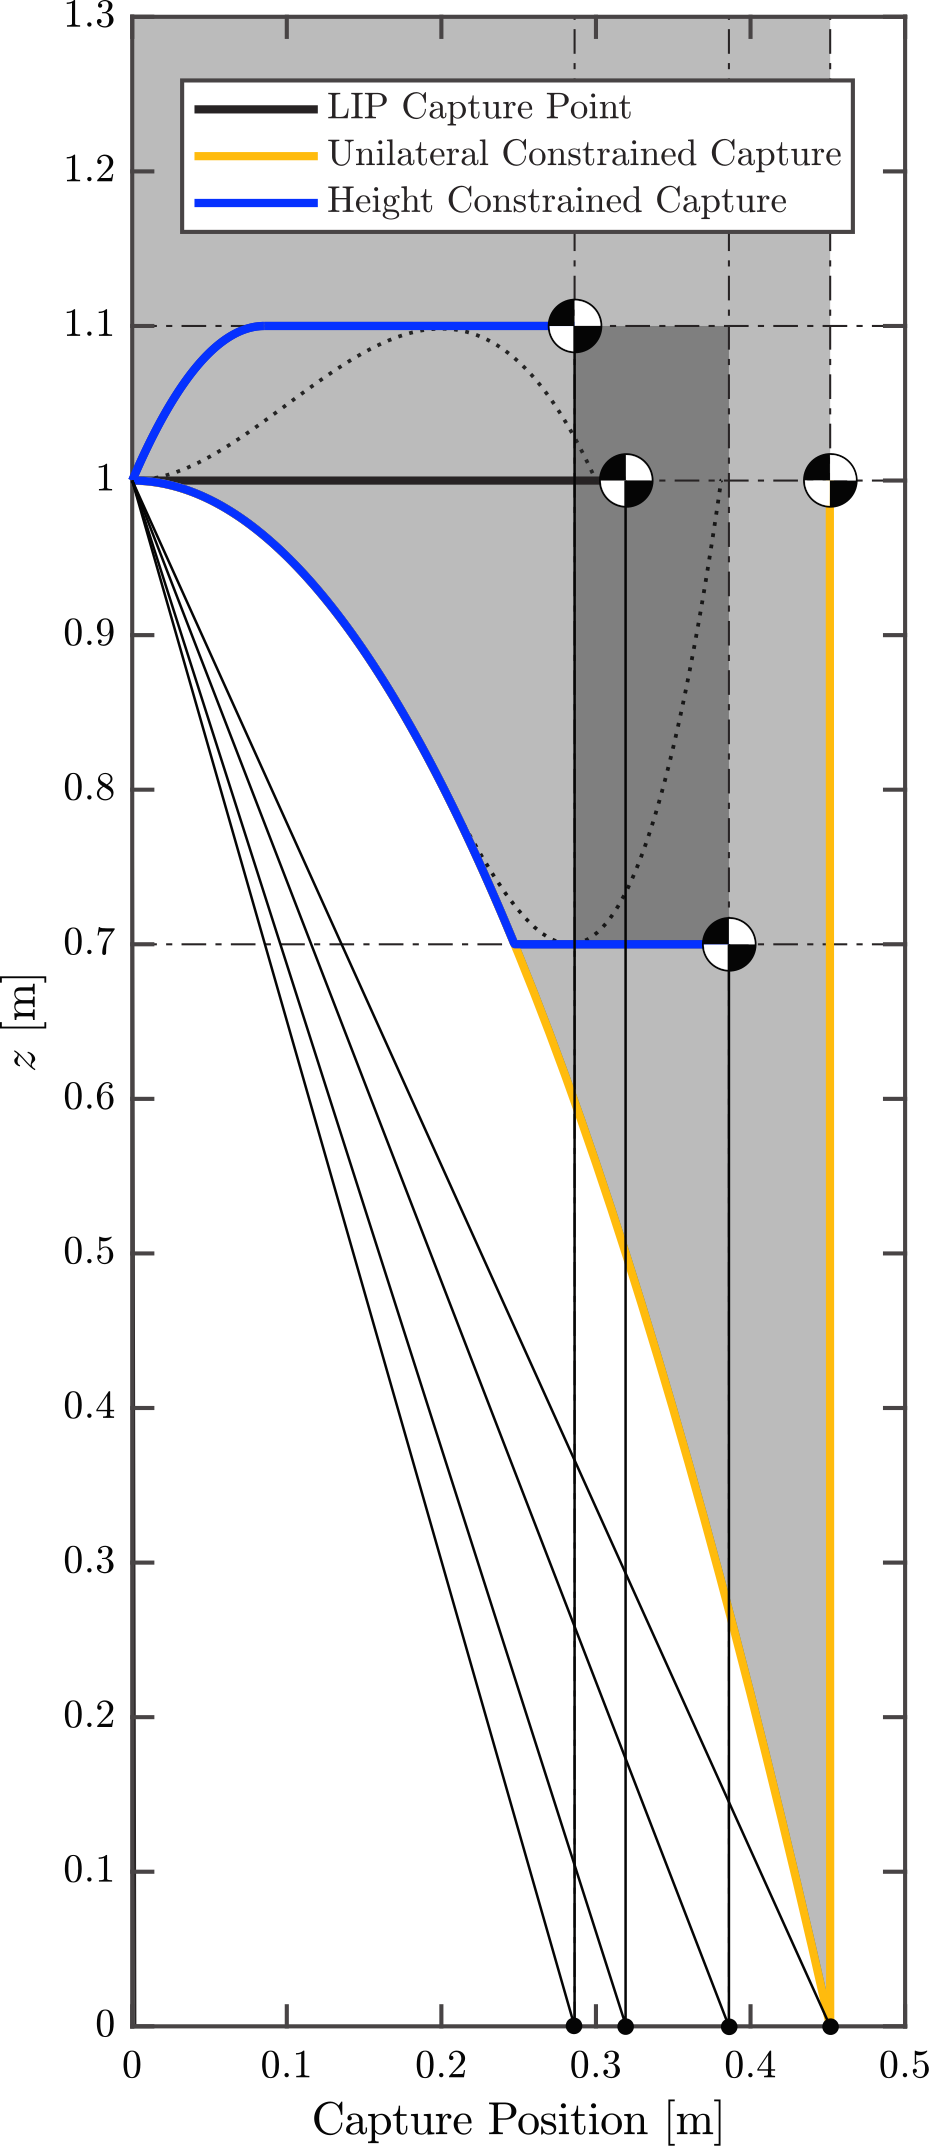
\includegraphics[width=3in]{STYLESTUFF/CPLimitsDark.png}
      \caption{Visualization of the analytic capture regions for $\dot{x}_0=1$ [m/s] and $\dot{z}_0=0$ [m/s]. The light gray area shows the unilateral contact constrained capture region (Section \ref{eq:xcpuni}). The dark gray area shows the height constrained capture region (Lemma \ref{lem:regionz})  for $0.7<z<1.1$ [m]. The dotted plots are made with the \textit{orbital energy controller} of \cite{koolen2016balance} and show that the final points are inside the height constrained region.}
      \label{fig:capregion}
\end{figure}

% Vertical Force
\section{Vertical Force Constraint}\label{sec:verticalforce}
As the height constrained capture region does not take torque limits into account, the \ac{VHIP} dynamics can be further constrained to narrow the gap between model and robot. If the assumption is made that the robot specific limitations on joint torques can be approximated with a minimum and maximum vertical force on the \ac{CoM}, constraints on the minimum and maximum vertical acceleration are added to the \ac{VHIP} dynamics. From Lemma 1, any vertical acceleration extremum at the earliest convenience will lead to staying closer to a height constrained bound. 
     
In \cite{pratt2006capture,stephens2007humanoid,koolen2012capturability}, a bang-bang control law is used to regulate the angular momentum in the body of model. Instead of using this strategy, a bang-bang control law is used to regulate the vertical acceleration:
\begin{equation}
	\ddot{z} = \ddot{z}_{c,1}H(t) - (\ddot{z}_{c,1} - \ddot{z}_{c,2})H(t-t_1) - \ddot{z}_{c,2}H(t-t_2),
\end{equation}
where $[\ddzcf,\ddzcs]$ are the first and second constant control inputs and have opposite signs. $H(\cdot)$ is the Heaviside step function and 
\begin{equation}
t_1=\sqrt{\frac{2(z_{const}-z_0)}{\ddzcf - \frac{\ddzcf^2}{\ddzcs}}},
\end{equation}
which is the solution of:
\begin{equation}
	z_0+\frac{1}{2}\ddzcf t_1^2 - \frac{1}{2}\frac{(\ddzcf t_1)^2}{\ddzcs}= z_{const},
\end{equation}
where $z_{const}=\zmin$ if $\ddzcf <0$ and $z_{const}=\zmax$ otherwise. The time $t_2=(1-\frac{\ddzcf}{\ddzcs})t_1$, as the second `bang` needs to drive the vertical velocity resulting from the first bang to zero. 
\begin{figure}
      \centering
      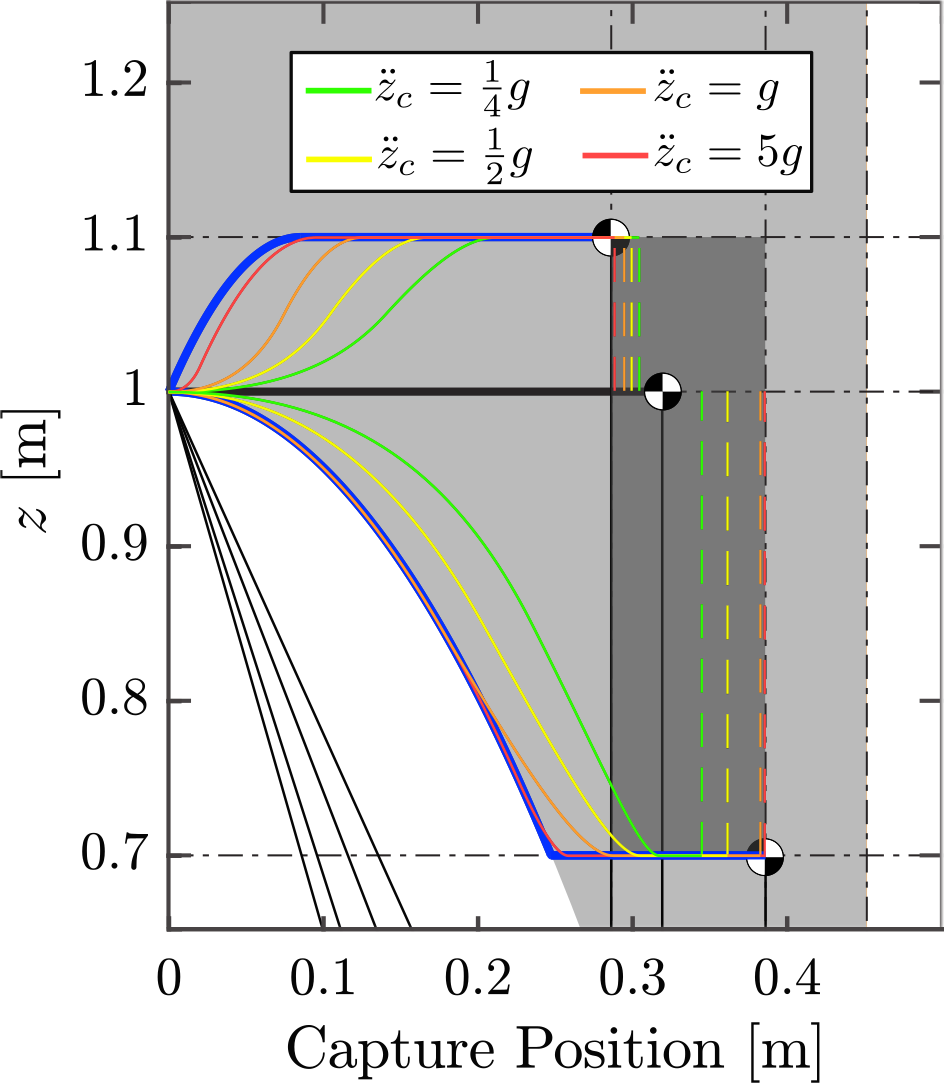
\includegraphics[width=3.2in]{STYLESTUFF/CPLimitsForce.png}
      \caption{Vertical acceleration constrained capture positions versus the height constrained bounds. The acceleration $\ddzc=|\ddzcf|=|\ddzcs|$ if $\ddzc \leq g$ and else the `bang' with the negative sign is set to $-g$.}
      \label{fig:zvsf}
\end{figure}

By inserting a constraint on vertical acceleration, the solution to a capture position is computed using a binary search. In this search, there is iterated over the initial position, given the initial velocity. The cost function used is $x^2$ at the time instance that $\dot{x}=0$.  If $\dot{x}$ is never zero, which happens when the point-mass crosses the pendulum base, the cost is set to a high value. The authors of \cite{gao2017increase} give analytic solutions using vertical acceleration, but consider a constant height in the model. For comparison with applied results later in this thesis, this constant height assumption is not considered. In Figure \ref{fig:zvsf}, simulation results are shown in perspective with the height constrained bounds. Note that when the bang-bang control inputs are larger, both trajectory and capture position come closer to the height constrained bounds.

%% Cap comparison
\section{Capturability Comparison}
In this section, a comparison is made between the presented capture positions and the \ac{CP}, as well as a comparison with the \ac{LIP} plus flywheel capture regions. As in \cite{pratt2006capture, stephens2007humanoid, koolen2012capturability}, a \textit{dimensional analysis} is performed on comparing the capture regions. The following parameters are used for dimensionless position and velocity:
\begin{equation}
	x' = \frac{x}{z_0}, \qquad \dot{x}' = \frac{1}{\sqrt{gz_0}}\dot{x}.
\end{equation}
The following dimensionless height and vertical acceleration are use for the \ac{VHIP}:
\begin{equation}
 z' = \frac{z}{z_0}, \qquad \ddot{z}'=\frac{\ddot{z}}{g}.
\end{equation}
And the following dimensionless in inertia and \ac{CoM} torque are used for the \ac{LIP} plus flywheel model:
\begin{equation}
I_y'=\frac{I_y}{mz_0^2}, \qquad \tau_y' = \frac{\tau_y}{mgz_0}.
\end{equation}
Instead of the \ac{CoM} torque, a dimensionless \ac{CMP} offset is used:
\begin{align}
	\xcmp' &=\frac{\xcmp}{z_0}=\xcop' + \delta \xcmp',\\
	\delta \xcmp' &=\tau_y',
\end{align}
where $\delta \xcmp'$ is the dimensionless \ac{CMP} offset. The dimensionless \ac{CoP} is assumed to be at a constant location.

\subsection{Comparison without Angular Momentum}\label{sec:capcomparenoinertia}
To make a comparison between the \ac{CP}, the height constrained capture positions and the vertical force constrained capture positions, the dimensionless vertical acceleration $\ddzc'$ of each `bang' for the vertical force constrained capture positions is set equal. For comparison, a rough estimate is made of realistic values of vertical forces that are achievable on both human and robot.

First, an approximation is made of what would be achievable for a human being. A human jumping vertically with maximum effort generates approximately $2mg$ ground reaction force \cite{linthorne2001analysis}. If the assumption is made that this value can also be used in recovery, we the value $\ddot{z}_c'=1$ can be taken for a human. Second, an approximation is made of what is possible on the robot. On hardware experiments on NASA's Valkyrie in Chapter \ref{chap:walking} is found that $\ddot{z}_c'=\frac{1}{4}$ is a well working value. Larger accelerations would result in the robot to shake and did not improve recovery. 

In the left plot in Fig. \ref{fig:caplimits}, the height constrained bounds are shown, together with our approximations of what is realistic for vertical acceleration constraints on a human and on the robot. Note how the capture positions relate differently under a minimum height constraint than under a maximum height constraint. Also note how the capture position linking to the approximation of allowed vertical acceleration for a robot, seems to approach a minimum and maximum value quite soon after changing height. The point $[1,1]$ in the plot is the \ac{CP}. In the right plot, the \textit{capture velocity} is shown. This is the initial velocity, after which the resulting capture point is equal to the \ac{CP}. The capture velocity is used later in this report for comparison with applied results.
\begin{figure}
      \centering
      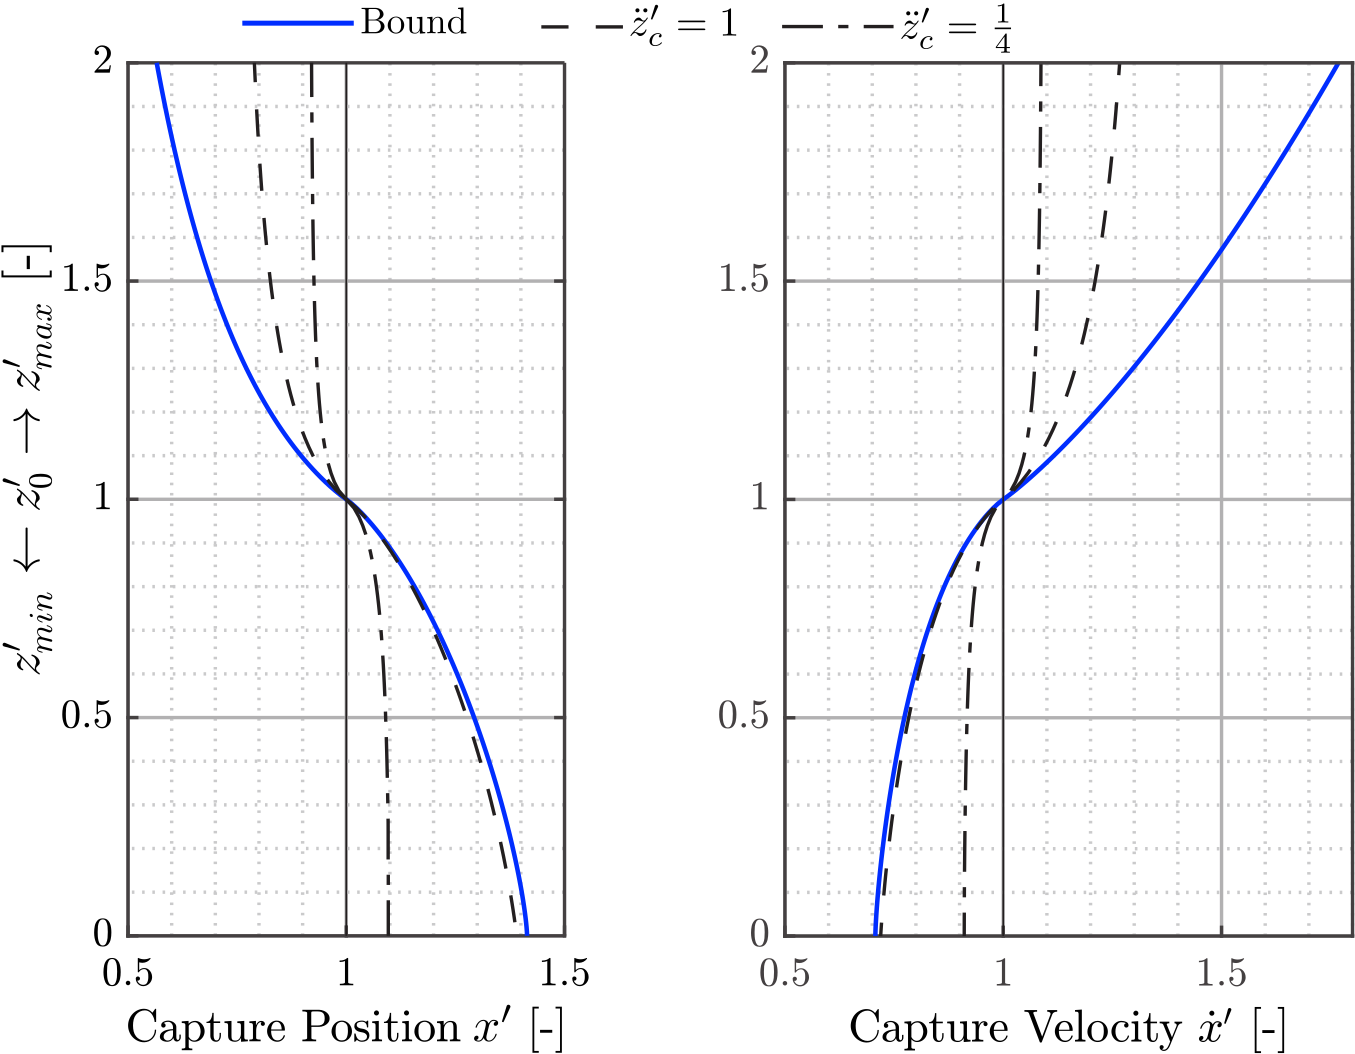
\includegraphics[width=5.2in]{STYLESTUFF/caplimits1.png}
      \caption{Plot of reachable dimensionless capture positions for $\dot{x}_0'=1$ (left) and capture velocities for $x_0' = 1$ (right). }
      \label{fig:caplimits}
\end{figure}
\subsection{Comparison with Angular Momentum}
An estimation of the effects of angular momentum strategies can be performed as in \cite{koolen2012capturability}. Angular momentum strategies, like a `hip' strategy, have a pay back time; any angular velocity generated by the strategy has to be driven back to zero before a physical limit is reached. Therefore, the body torque can be estimated with a bang-bang control law.  Considering a \ac{LIP}, as proposed in the work mentioned, the following method is used to account for angular momentum:
\begin{equation}
\delta\xcmp' = (1-2e^{-\delta \tbang'}+e^{-2\delta \tbang'})\delta \xcmpmax',
\end{equation}
\begin{figure}
\centering
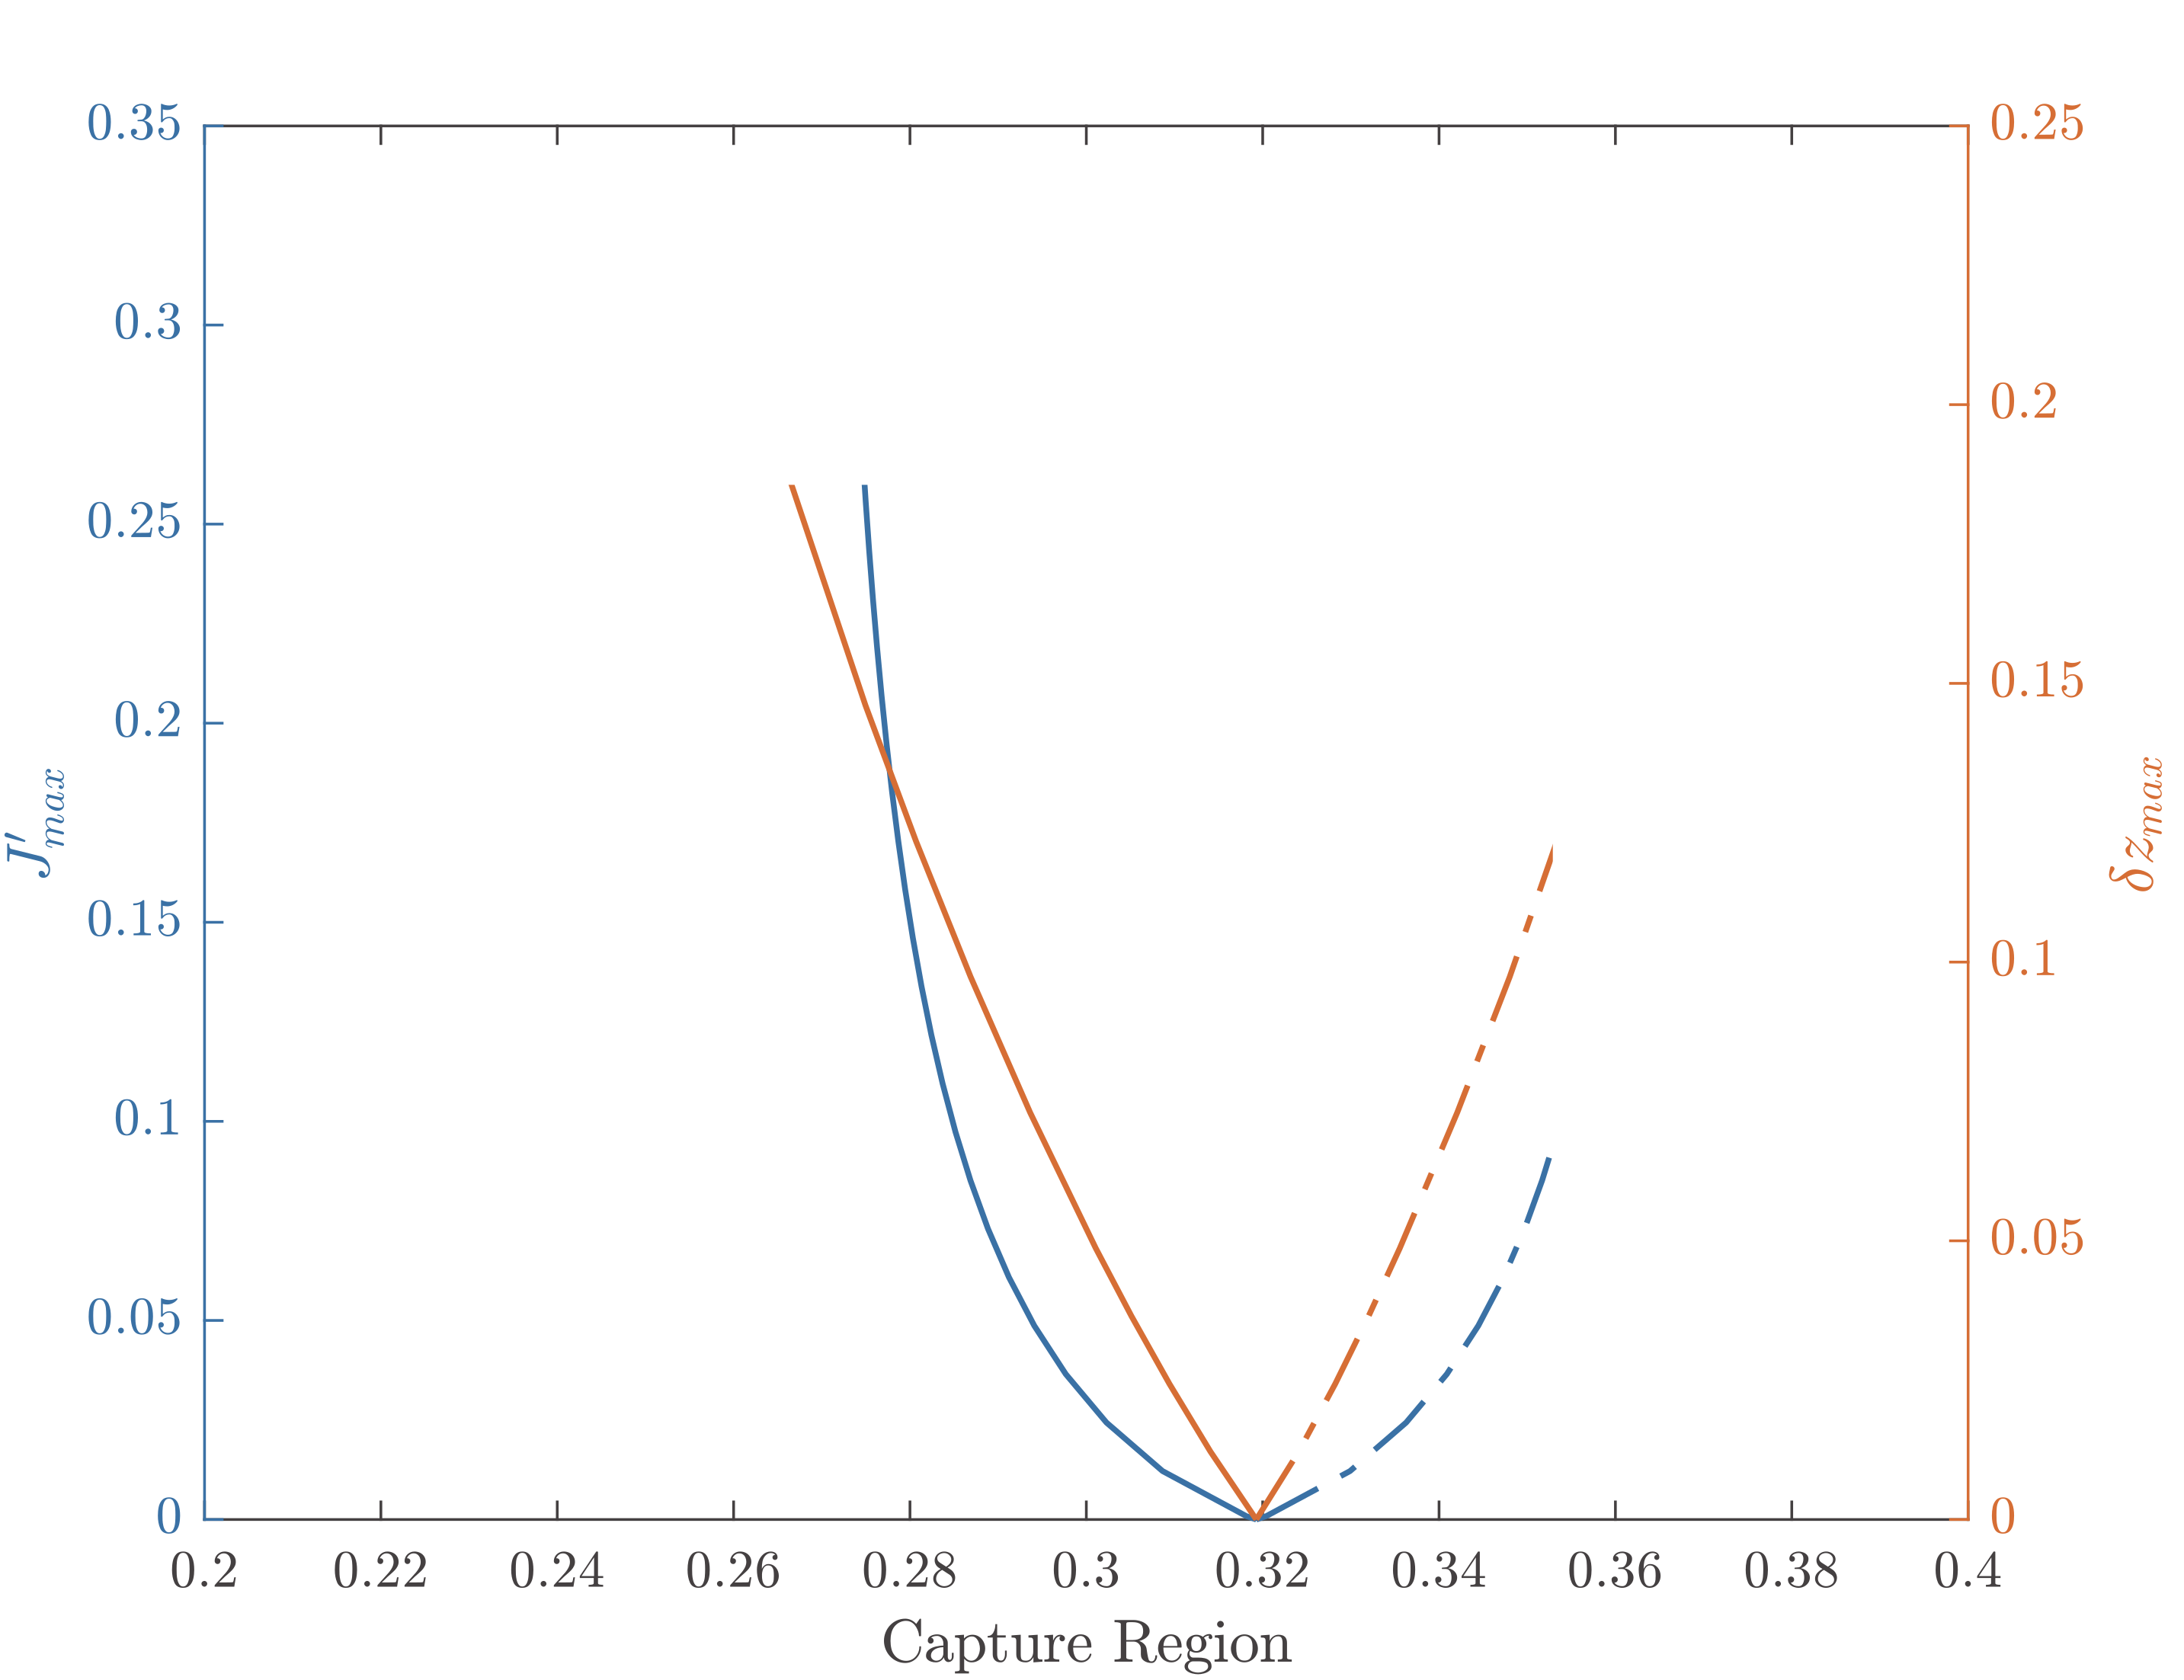
\includegraphics[width=0.9\textwidth]{STYLESTUFF/capcompare.png}
\caption{Comparison of capture region with angular momentum versus vertical force constrained capture. $\delta \zmax' =\delta \zmin'$ and $I_y' = \frac{1}{6}$. The solid plots show the first bound on the region and the dotted plots the second bound.}
\label{fig:capcompare}
\end{figure}
where $\delta \xcmpmax'$ is the maximum dimensionless offset of the \ac{CMP} with the \ac{CoP} and $\delta \tbang'$ is the time of each ``bang'' of the control law. The average dimensionless \ac{CMP} offset to account for in computation of the \ac{CP} is $\delta \xcmp'$. The time $\delta \tbang'$ can be determined by:

\begin{equation}
\delta \tbang' = \sqrt{\frac{I_y'\theta_{max}}{\delta \xcmpmax'}},
\end{equation}
where $\theta_{max}$ the maximum allowed body lunge compared to the vertical. Note that $I_y'=0$ for a point-mass and $I_y'=1$ for a disc with all its mass on the edge, with its radius equal to the \ac{CoM} height above the ground. 

A rough estimate can be made of the dimensionless inertia of a human used in recovery. The assumption is made that the hip is the \ac{CoM} position and that the total body length is two times the \ac{CoM} height. Furthermore, only the body above the hip is assumed to be used in recovery, which is modeled as a beam with half the total body mass rotating around an end: $I_{beam} = \frac{1}{3}(\frac{1}{2}m)L^2$. Note that the length $L$ is equal to the \ac{CoM} height $z$. Those assumptions result in the following dimensionless inertia:
\begin{equation}
	I_y' = \frac{\frac{1}{3}(\frac{1}{2}m)z^2}{mz^2} = \frac{1}{6}.
\end{equation}
Even though the inertia used in recovery is approximated with a calculation based on a beam, still a flywheel model is assumed. Rotation of a beam around its end would, in the case of a `hip' strategy, change the \ac{CoM} height of the system and would violate the \ac{LIP} model.

In \figref{fig:capcompare} the force constrained capture regions are compared with \ac{LIP} with flywheel capture regions. The maximum allowed vertical \ac{CoM} height change $\delta \zmax' =0.065$ is approximately the same value as is used on NASA's Valkyrie later in this report.

%% Discussion
\section{Discussion}
In this chapter, different capture positions and capture regions for the \ac{VHIP} model are introduced. By comparing the capture positions, it can be observed how the addition of a constraint on the model can affect the capture region. Also, a high level comparison is made with angular momentum strategies.

Combination of height variation and angular momentum for balance recovery has two aspects worth mentioning. First, the \ac{GRF} in the phases with low or zero leg force will almost be orthogonal to the gravity vector if a hip torque is applied, which can cause slipping if ground friction is limited. Second, with lunging of the upper body, the \ac{CoM} will lower. In cases where height is increased for balance, this strategy is thus conflicting with use of angular momentum. Even maintaining a constant \ac{CoM} height may be difficult with lunging the upper body.

Friction cone..